\newcommand{\NWtarget}[2]{#2}
\newcommand{\NWlink}[2]{#2}
\newcommand{\NWtxtMacroDefBy}{Fragment defined by}
\newcommand{\NWtxtMacroRefIn}{Fragment referenced in}
\newcommand{\NWtxtMacroNoRef}{Fragment never referenced}
\newcommand{\NWtxtDefBy}{Defined by}
\newcommand{\NWtxtRefIn}{Referenced in}
\newcommand{\NWtxtNoRef}{Not referenced}
\newcommand{\NWtxtFileDefBy}{File defined by}
\newcommand{\NWtxtIdentsUsed}{Uses:}
\newcommand{\NWtxtIdentsNotUsed}{Never used}
\newcommand{\NWtxtIdentsDefed}{Defines:}
\newcommand{\NWsep}{${\diamond}$}
\newcommand{\NWnotglobal}{(not defined globally)}
\newcommand{\NWuseHyperlinks}{}
\documentclass{article}
\usepackage{graphicx}
\usepackage{pstricks}
\usepackage{listings}
\begin{document}
Daniel Hulseman Ted Wang Sahil Chopra Weihan Zhang
\section{Specification}
We will be making an app that will prompt the user for either/or a zip code or town name, and return the weather for that area. The weather for the area will be represented by a picture.
\\\\
Goals:\\
- User will be able to choose which area he/she wants to check the weather\\
- 1-7 day forecast will be returned along with other information, such as a preference of Celsius or Fahrenheit\\
- Pictures and sound appropriate for the weather\\
\\
Things we'd like to do:\\
- Save what the weather was last time you ran the program\\
- Custom animation for the weather using FLTK\\
- Choose which day you want to see the weather for\\
- Mute button!\\

\begin{pspicture}(-5,-5)(5,5)
\psframe[fillstyle=solid,fillcolor=lightgray](-5,-5)(5,5)
\psframe[fillstyle=solid,fillcolor=white](-1,3)(1,4)
\rput(-2.5,3.5){Enter area code:}
\rput(0,3.7){94538}
\psframe[fillstyle=solid,fillcolor=darkgray](2,3.5)(3,4)
\rput(2.5,3){Button!}
\psframe[fillstyle=solid,fillcolor=cyan](-3,-3)(3,2.5)
\pscircle[fillstyle=solid,fillcolor=yellow](0,-.5){1.25}
\rput(0,-3.25){Sunny! 75F}
\end{pspicture}

\section{Analysis}
IPO: Inputs are the zip code from the user, and the current weather taken from the internet, in addition to a preference of Fahrenheit or Celsius. Output is the weather, temperature, humidity, time, etc, represented by pictures/animation and sound. Process could entail a timer from the last time you requested weather, and conversions from Fahrenheit to Celsius or vice versa and checking to get the appropriate picture/sound for the weather.\\\
Example:\\
-User enters 94538 as the zip code, and sets Fahrenheit\\
-Program displays a sun, while birds chirp and peaceful music plays. Displays 77F.\\
-Program begins to count how long ago he requested the weather.\\
Example 2 (invalid zip code):\\
-User enters 1234 as the zip code.\\
-Program displays a red X where the weather would have been and displays "Invalid zip code" where the temperature would have been.\\
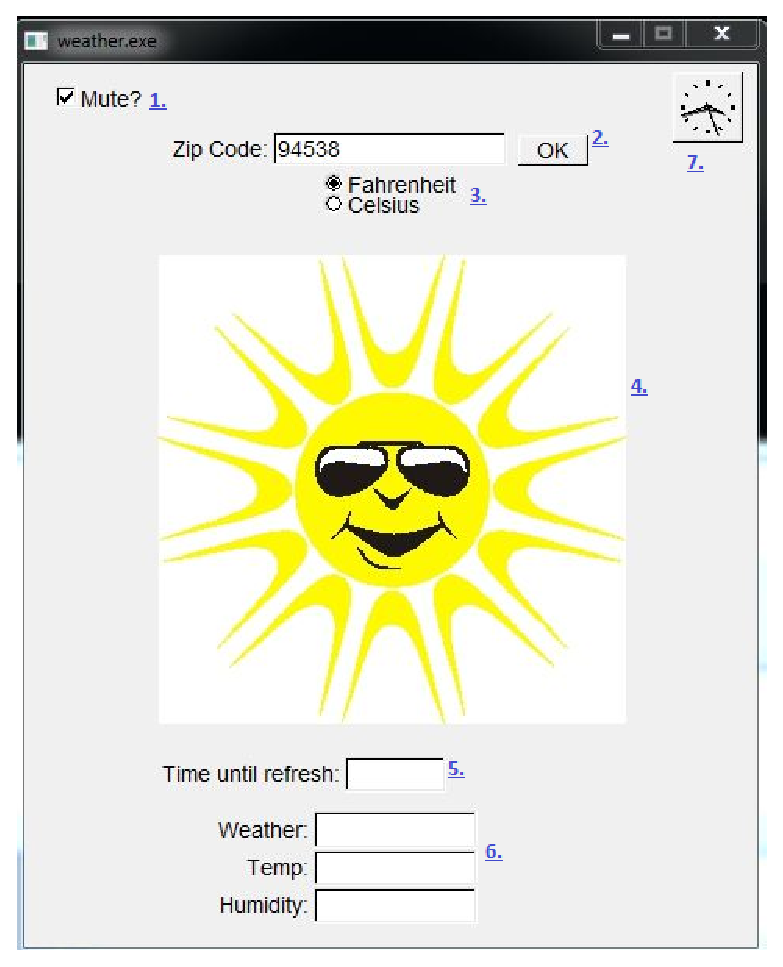
\includegraphics[bb=0 0 480 600]{GUIwip.eps}
\\
\begin{enumerate}
\item Mute function: Input is the check box and whether or not it is checked. Output is either muted sound or allowed sound. We aren't sure how to do this yet so help is appreciated. 
\item This is the meat of the program. The user must input a zip code and hit the OK button when ready. Output is the weather represented symbolically in function 4 and details in function 6. Process retrieving the data from a database. \\
\item Temperature preference: Input is done via the radial buttons picking the preferred unit of temperature. Output is displayed in function 6 giving you your preferred units. Process is done by calculating fahrenheit from celsius or vice versa depending on our database's units.\\
\item Image selection: Input is acquired by function 2's output. Output is the appropriate image according to the weather. The process is similar to lab13: there are actually multiple images overlayed on top of each other. In order to display the appropriate weather the program must display the image with the appropriate value and hide all the others that don't apply.\\
\item Refresh Timer: Input once again comes from function 2's OK button. Output is simply time counting down from when that button was pressed until data is re-retrieved. This process is done by using the FLTK(?) timeout function counting down from when this button was pressed, and then returning data for the same zip code again. 
\item Weather details: Input is acquired from data from the internet acquired from function 2 and also temperature determined by function 3.Output is details about weather conditions from this database. Process is to acquire data from the internet.
\item Time (relative to the zipcode): Function 2 provides the input for this function. Output is time relative to the area that we specified. For example, if the area code is for Fremont, it display Pacific standard time. Process is to retrieve data from the internet relevant to this.
\end{enumerate}

\section{Design}
We wrote a cpp file that retrieves data, finds data, and converts data from internet first so we'll know what and how to do inside FLuid. 
Then used FLuid to create the cxx source file. Here is what is produced:

\section{Implementation}
\lstinputlisting[language=c++]{weather.cxx}

\section{Test}
%\includegraphics[bb= ]{ .eps}
\end{document}